\documentclass[10pt]{article}

\usepackage{fancyhdr}
\usepackage{geometry}
\usepackage{chemfig}
\usepackage{amsmath}
\usepackage{pgfplots}
\usepackage{rotating}
\usepackage{multicol}
\usepackage{tikz}
\usepackage{multicol}
\usetikzlibrary{arrows,positioning,shapes.geometric}
\usepgfplotslibrary{polar}

\geometry{
    top=20mm,
    bottom=30mm,
    left=20mm,
    right=20mm
}

\fancyfoot[L]{
    \begin{turn}{180}
        \begin{minipage}{0.4\linewidth}
            \begin{flushright}
                \begin{multicols}{2}
                    \emph{written exclusively under the influence}
                    \begin{turn}{90}
                    \chemfig{[,0.4]*6(([,0.5]=)-([6,0.7]-)-*5(-=-([:60, 0.7]-)-=)--([,0.5]=)-([:150, 0.7]-)-)}
                    \end{turn}
                \end{multicols}
            \end{flushright}
        \end{minipage}
    \end{turn}
}

\pagestyle{fancy}

\renewcommand{\headrulewidth}{0pt}



\begin{document}

\title{\underline{A treatise on non-aquatic gastropod Mollusca, a.k.a. \emph{snails}}}
\author{Aayush Bajaj}
\date{\today}
\maketitle

\tableofcontents

\dotfill
\bigbreak

\section*{Definitions}

    \begin{flushright}
    \begin{minipage}{8cm}
        \begin{flushleft} \emph{If you wish to converse with me define your terms.} \end{flushleft}
        \begin{flushright}--- Voltaire\end{flushright}
    \end{minipage}
    \end{flushright}

    Snails are defined as gastropods that have a shell. Gastropods are a \underline{class} of invertebrates which include slugs, squids, octupuses \emph{and} snails. These gastropods belong to a \textbf{larger} \underline{phylum} of animals called \emph{Mollusca}.

\section*{Classifications}

    The gastropod class includes both aquatic and non-aquatic snails and are the most diverse class of \emph{Molluscs}, residing in \textbf{every} marine environment from high-energy surge zones to ocean floorbeds.

    Restricting our study to \emph{non-aquatic} gastropods brings us to 2 particular \underline{families}; the \textbf{prosobranchia} and the \textbf{pulmonata}.

    \subsection*{Prosobranchia}
        
    \subsection*{Pulmonata}


    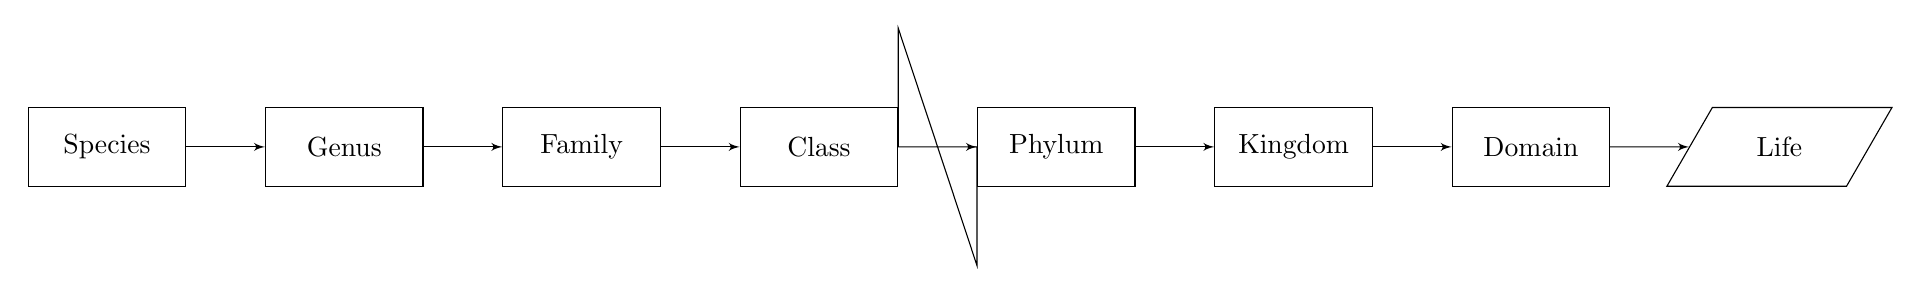
\begin{tikzpicture}[>=latex']
        \tikzset{block/.style= {draw, rectangle, align=center,minimum width=2cm,minimum height=1cm},
        rblock/.style={draw, shape=rectangle,rounded corners=1.5em,align=center,minimum width=2cm,minimum height=1cm},
        input/.style={ % requires library shapes.geometric
        draw,
        trapezium,
        trapezium left angle=60,
        trapezium right angle=120,
        minimum width=2cm,
        align=center,
        minimum height=1cm
    },
        }
        \node [block]  (start) {Species};
        \node [block, right =1cm of start] (acquire) {Genus};
        \node [block, right =1cm of acquire] (rgb2gray) {Family};
        \node [block, right =1cm of rgb2gray] (otsu) {Class};
        \node [block, right =1cm of otsu] (gchannel) {Phylum};
        \node [block, right =1cm of gchannel] (closing) {Kingdom};
        \node [block, right =1cm of closing] (NN) {Domain};
        \node [input, right =1cm of NN] (limit) {Life};
        \node [coordinate, below right =1cm and 1cm of otsu] (right) {};  %% Coordinate on right and middle
        \node [coordinate,above left =1cm and 1cm of gchannel] (left) {};  %% Coordinate on left and middle

%% paths
        \path[draw,->] (start) edge (acquire)
                    (acquire) edge (rgb2gray)
                    (rgb2gray) edge (otsu)
                    (otsu.east) -| (right) -- (left) |- (gchannel)
                    (gchannel) edge (closing)
                    (closing) edge (NN)
                    (NN) edge (limit)
                    ;
    \end{tikzpicture}

\section*{Habitat}
    
\section*{Behaviours}

\newpage

\begin{multicols}{2}

    \begin{minipage}{0.4\textwidth}
    \section*{Facts}
        Snails are hermaphrodites, they all have pp
    \end{minipage}

    \begin{flushleft}
    \begin{minipage}{0.5\textwidth}
    \section*{Mathematics}

        \def\spiral#1{%
          \pgfmathparse{int(#1)}%
          \ifnum\pgfmathresult>0
            \begin{scope}[shift={(1,1)}, rotate=90, scale=1/1.6180339887]
              \spiral{#1-1}
            \end{scope}
            \draw [black] (0,0) arc (270:360:1);
          \fi
        }

        Let us briefly consider the length of an ordinary garden snail's shell.
        Approximating the shell to abide by the natural shape of the \emph{Golden Spiral} we may then use \[ l = \int^{\theta_1}_{\theta_0} \sqrt{[f(\theta)]^2 + [f'(\theta)]^2} \, \mathrm{d}\theta .\]
        

        \begin{turn}{90}
        \tikz[scale=3]{\spiral{50}}
        \end{turn}


        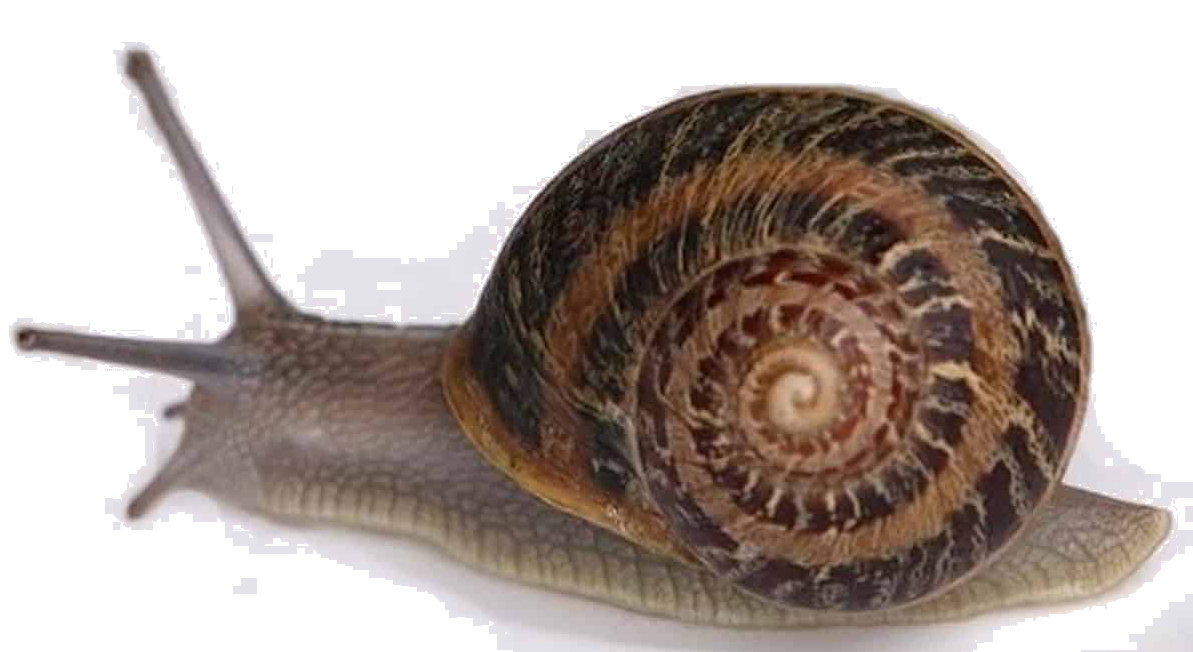
\includegraphics[width=\textwidth]{img/snail.png}
    \end{minipage}
    \end{flushleft}

\end{multicols}

\section*{Glossary}
Phylum
Herbivore, Omnivore, Carnivore
\section*{References}



Snails are defined as gastropods that have a shell. 

This shall be a fun exercise. I will need to learn how to produce a tree diagram in \LaTeX{} as well as a TikZ picture of a golden spiral overlaid atop a snail (at the very least).

To accomplish the latter I shall leverage the arc length of a curve as \(\theta_1 \rightarrow \infty\) for \(l\), where


Then for a given curve such as \(r = e^\frac{\theta}{10}\):
\begin{center} % you could probably tell tikz to center?
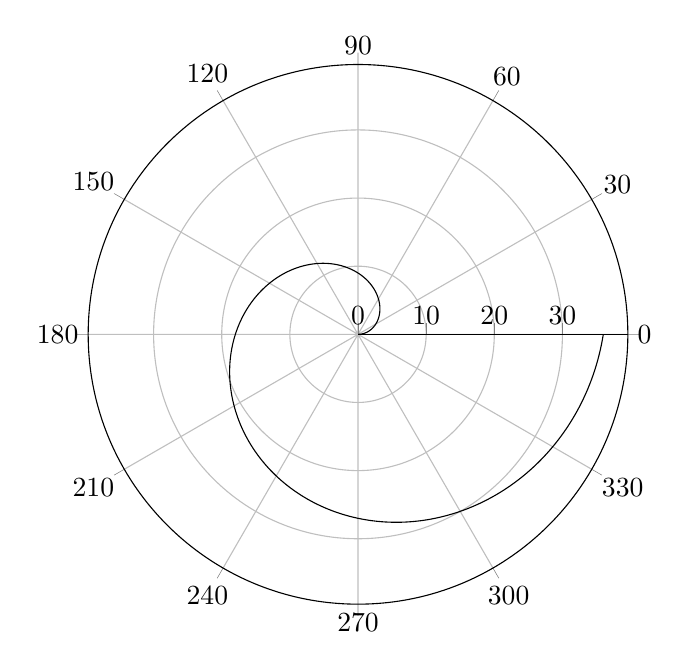
\begin{tikzpicture}
    \begin{polaraxis}
        \addplot[domain=0:360, samples=300]{0.10*x};
    \end{polaraxis}
\end{tikzpicture}
\end{center}

The length of the arc is:
\begin{align*}
    l &= \int^{\theta_1}_{0} \sqrt{(e^{-\frac{\theta}{10}})^2 + (-\frac{1}{10}e^{-\frac{\theta}{10}})^2}\mathrm{d}\theta\\
    &= \int^{\theta_1}_{0} \sqrt{(1+\frac{1}{100})e^{-\frac{2\theta}{10}}} \mathrm{d}\theta\\
    &= \frac{\sqrt{101}}{10} \int^{\theta_1}_0 e^{-\frac{\theta}{10}}\mathrm{d}\theta\\
    &= \sqrt{101}(1 - e^{-\frac{\theta_1}{10}}).\\
    &= \sqrt{101} \text{ (as \(\theta_1 \rightarrow \infty\))}
\end{align*}

\end{document}
